\documentclass{report}

\usepackage{mathtools, amsthm, amsmath, amssymb}
\usepackage{babel}
\usepackage[thaifont=TH Sarabun New]{thaispec}
\usepackage{biblatex}
\addbibresource{Project.bib}

\title{แบบจำลองทางคณิตศาสตร์\\การขายครัวซองค์}
\author{    
\begin{tabular}{ll}
	นางสาวอนาตี มะหะหมัด 116510901022-3\\นางสาวอจิรวดี จันทวรรณ 116510901026-4\\นายอภิชาติ ทิพยโอสถ 116510901020-7
\end{tabular}\\ 
\\
เสนอ\\
ดร.รัฐพรหม พรหมคำ\\
ผู้ช่วยศาสตราจารย์ ดร.วงศ์วิศรุต เขื่องสตุ่ง\\
ผู้ช่วยศาสตราจารย์ ดร.ภคีตา สุขประเสริฐ\\
\\
สาขาวิชาคณิตศาสตร์ คณะวิทยาศาสตร์และเทคโนโลยี\\
มหาวิทยาลัยเทคโนโลยีราชมงคลธัญบุรี
}
\date{1 มีนาคม 2567}

\begin{document}
\maketitle
\tableofcontents
\listoftables
\listoffigures

\pagebreak

\begin{center}
\textbf{บทคัดย่อ } 
\end{center}
แบบจำลองทางคณิตศาสตร์การทำร้านครัวซองค์ เป็นแบบจําลองที่ถูกสร้างขึ้นเพื่อวิเคราะห์และวางแผนในการลงทุนรวมถึงกลยุทธ์ทางการเงินต่างๆ โดยการคํานวณต้นทุนในการทําครัวซองค์เพื่อให้ถูกขายออกให้หมดและไม่ขาดทุนในแต่ละครั้ง และยังสามารถคาดการณ์ถึงอนาคตว่าจะได้กำไรเมื่อขายในเดือนที่เท่าไหร่

\begin{center}
\chapter{บทนำ}
\end{center}
\section{ที่มาและความสำคัญ}
โครงงานฉบับนี้ได้จัดทําขึ้นเพื่อประโยชน์สําหรับศึกษาและเรียนรู้ในการลงทุนทําร้านครัวซองค์โดยได้ทําการรวบรวมข้อมูลเกี่ยวกับการเริ่มทําธุรกิจ รวมทั้งกลยุทธ์ทางการเงิน \par
แบบจําลองทางคณิตศาสตร์การทําร้านครัวซองค์จัดทําขึ้นสําหรับผู้ที่สนใจจะลงทุนในธุรกิจดังกล่าว ซึ่งแบบจำลองที่ออกแบบมาเพื่อวางแผนในการลงทุน โดยการคํานึงถึงผลกําไรในอนาคต\par
ดังนั้นคณะผู้จัดทําหวังเป็นอย่างยิ่งว่าแบบจําลองคณิตศาสตร์เล่มนี้ได้รวบรวมเนื้อหาที่เป็นประโยชน์แก่ผู้สนใจ และทําความเข้าใจลักษณะของการลงทุนทําธุรกิจและกลยุทธ์ทางการเงินตลอดจนทําการศึกษาเพิ่มเติม เพื่อนำไปจัดทำต่อยอดได้ในเชิงธุรกิจ ที่มีความเหมาะสมในเชิงปฏิบัติมากขึ้น
\section{วัตถุประสงค์}
\begin{itemize} 
	\item เพื่อให้มีความเข้าใจในการลงทุนทําธุรกิจร้านครัวซองค์
	\item เพื่อเสริมสร้างประสบการณ์ทางด้านวิชาชีพ
\end{itemize}
\section{ประโยชน์ที่คาดว่าจะได้รับ}
\begin{itemize}
    \item ได้รับกลยุทธ์ทางด้านการลงทุนเพิ่มขึ้น
    \item เพิ่มขีดความสามารถในการทำงานอย่างเป็นระบบ
\end{itemize}

\section{ขอบเขต}
\begin{itemize}
    \item{การใช้กลยุทธ์การตลาดที่เหมาะสมเช่น การโฆษณาผ่านสื่อต่างๆ การใช้โซเชียลมีเดีย เว็บไซต์ หรือแคมเปญโปรโมทสินค้า เป็นต้น สามารถช่วยเพิ่มยอดขายได้ }
\end{itemize}

\chapter{ความรู้ทั่วไป}
\section{ครัวซองค์}มีที่มาจริงๆจากสงครามระหว่างจักรวรรดิออตโตมันและกรุงเวียนนาประเทศออสเตรียโดยมีความรุนแรงถึงขั้นปิดล้อมกรุงเวียนนาเลยทีเดียวแต่สุดท้ายชาวเวียนนาก็สามารถเอาชนะสงครามครั้งนี้ได้ และเพื่อเป็นการเฉลิมฉลองชัยชนะครั้งนี้ ชาวเวียนนาจึงได้ริเริ่มอบขนมปังที่มีลักษณะคล้ายรูปพระจันทร์ครึ่งเสี้ยวซึ่งก็นํามาจากสัญลักษณ์บนธงของประเทศของศัตรูและใช้ชื่อเรียกว่าขนมคิปเฟล (Kipferl) นั่นเอง ด้วยชัยชนะของสงครามนี้จึงทำให้เกิดวันครัวซองโลก (World's Croissant Day) ซึ่งตรงกับวันที่ 30 มกราคมของทุกปี (สามารถดูข้อมูลเพิ่มเติ่มได้จากอ้างอิงข้างต้น) \cite{YOYO} เพื่อเป็นการรำลึกถึงชัยชนะในสงครามระหว่างจักรวรรดิออตโตมันและกรุงเวียนนาเสมอมา
ประเภทของครัวซองค์ (สามารถดูข้อมูลเพิ่มเติ่มได้จากอ้างอิงข้างต้น) \cite{KIKI}
\begin{enumerate} 
	\item ครัวซองต์ตรง (straight  Croissant) หรือที่นิยมเรียกกันว่าครัวซองต์แบบธรรมดา (Plain Croissant) ครัวซองค์แบบเบสิกที่จะมีจุดเด่นอยู่ที่เท็กซ์เจอร์แบบกรอบนอกนุ่มใน นิยมทานกันแบบไม่มีไส้ และนิยมทานเป็นมื้อเช้าคู่กับชาหรือกาแฟร้อน ๆ
	\item ครัวซองต์แบบพวงกุญแจ (Crescent Croissant) ครัวซองค์รูปทรงคล้ายพระจันทร์เสี้ยวหรือครัวซองค์แบบดั้งเดิมนั่นเอง ครัวซองค์รูปแบบนี้เป็นที่นิยมจะหาทานได้ง่าย
	\item ครัวซองต์รูปพลอย (Diamond Croissant) รูปทรงยอดฮิตในไทยขณะนี้ ครัวซองค์ทรงนี้จะค่อนข้างพอง ๆ มีเท็กซ์เจอร์ที่กรอบ และสามารถนำไปประยุกต์ใส่ไส้ได้อย่างหลากหลาย
\end{enumerate}
สิ่งที่ทำให้ครัวซองค์ทั้ง 3 แบบนี้แตกต่างกันขึ้นอยู่กับวัตถุดิบที่ใช้ เช่น ครัวซองต์แบบพวงกุญแจ จะเน้นการใช้มาร์การีน เนยหรือไขมันเทียม ส่วน ครัวซองต์ตรง และ ครัวซองต์รูปพลอย จำเป็นต้องใช้แต่เนยแท้เท่านั้น (สามารถดูข้อมูลเพิ่มเติ่มได้จากอ้างอิงข้างต้น) \cite{KIKI}\par
\begin{figure}[h!]
	\centering
	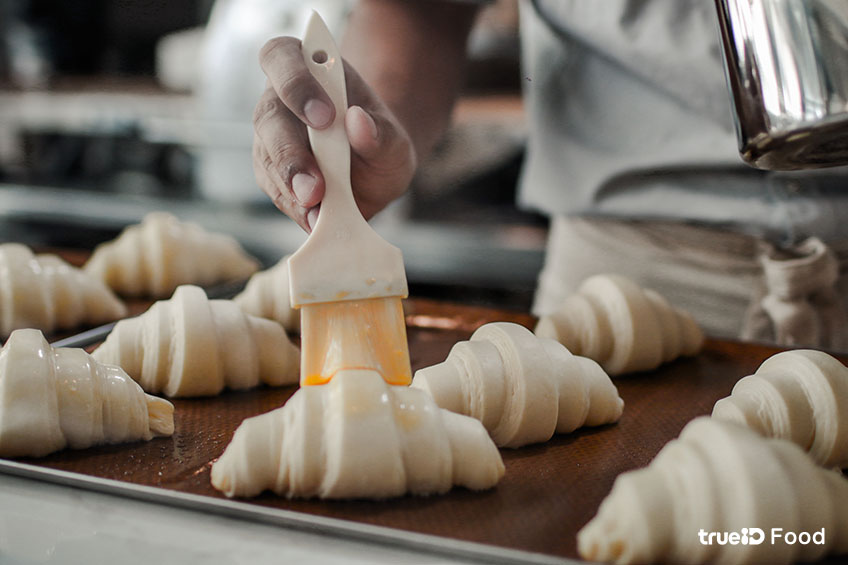
\includegraphics[scale=0.25]{OIP.jpg}
	\caption{ภาพครัวซองค์ \cite{POPO}}
	\label{fig:graph1}
\end{figure}

\textbf{วิธีการทําครัวซองค์}  \par โดยการทำครัวซองค์จะมีระยะเวลาในการเตรียมแป้ง 2 ชั่วโมง และระยะเวลาในการอบ 30 นาที (สูตร 24ชิ้น)\par

วัตถุดิบ
\begin{itemize}
	\item นมอุ่นๆ 1½ ถ้วยตวง
	\item น้ำตาลทรายไม่ขัดสี ¼ ถ้วยตวง
	\item ยีสต์แห้ง 3¼ ช้อนชา
	\item แป้งอเนกประสงค์ 3¼-4 ถ้วยตวง
	\item เกลือป่น 1 ช้อนโต๊ะ
	\item เนยจืด แช่เย็น 1½ ถ้วยตวง
	\item ไข่ไก่ 1 ฟอง
\end{itemize} \par
วิธีทำ 
\begin{enumerate} 
	\item ใส่นม น้ำตาล และยีสต์ลงในถ้วยผสม ใข้ตะกร้อคนให้เข้ากัน ทิ้งไว้ 5-10นาที(ถ้ายีสต์ทำงานดี จะเห็นเป็นฟองลอยอยู่ด้านบน)หลังจากนั้นนำไปเทลงในหม้อผสม 
	\item เติมแป้ง และเกลือลงไปในหม้อผสม ใช้หัวตีตะขอ ตีด้วยความเร็วต่ํา ประมาณ 5นาที จนเนื้อเนียนและนิ่ม(ถ้าเเป้งโดว์เหลวไปจะติดที่ขอบหม้อ ให้ค่อยๆเติมแป้งทีละ 1ช้อนโต๊ะ จนกว่าเนื้อจะเนียนดี)
	\item เมื่อแป้งโดว์ได้ที่แล้ว นำมานวดต่อบนโต๊ะด้วยมืออีก 2-3 นาที
	\item เมื่อเนื้อเนียนดีแล้ว ใส่กลับไปในหม้อ ปิดด้วยพลาสติก พักไว้ในตู้เย็น 1 ชม.
	\item ขณะที่พักแป้ง มาเตรียมเนยโดยเรียงเนยเป็นแท่งๆบนพลาสติกแรป ค่อยๆกดและรีดเนยไปมาทั้งสองด้าน ให้เป็นทรงสี่เหลี่ยมผืนผ้าขนาดประมาณ 8×5 นิ้ว จากนั้นห่อด้วยพลาสติกแล้วพักไว้ในตู้เย็น
	\item หลังจาก 1 ชม. เตรียมรีดแป้งกับเนยให้เข้ากัน โดยโรยแป้งบางๆบนโต๊ะ แล้วนำแป้งโดว์มารีดให้ได้ขนาดประมาณ 16×10 นิ้ว แล้ววางเนยไว้ตรงกึ่งกลางของแป้ง จากนั้นให้พับแป้งทีละด้าน จากขอบมาตรงกลาง จะได้รูปซองจดหมาย ใช้แปรงสะอาดปัดแป้งส่วนเกินออกให้หมด
	\item หมุนแป้งให้ด้านแคบอยู่ฝั่งเรา จากนั้นเริ่มรีดแป้งออกให้ได้ 16×10 นิ้ว อีกครั้ง แล้วพับแป้งเป็นรูปซองจดหมายแบบเดิม จากนั้นห่อด้วยพลาสติกแรปแล้วพักในตู้เย็นอีก 1 ชม. ขั้นตอนนี้คือ การพับครั้งที่ 1
	\item พอครบ 1 ชม. ก็นำแป้งออกทำซ้ำขั้นตอนเดิม ทำแบบนี้ 3 รอบ ก็จะได้การพับ 5 รอบ
	\item เมื่อพับครบแล้ว ให้แช่เย็นไว้ข้ามคืนหรืออย่างน้อย 8 ชม.
	\item เริ่มขั้นตอนการขึ้นรูป โดยตัดแป้งที่พักไว้แล้วออกมาครึ่งนึง (ส่วนที่เหลืออีกครึ่งนึง แช่ฟรีซเก็บไว้)
	\item เพื่อให้การทำงานง่ายขึ้น เราสามารถแบ่งแป้งออกเป็น 3 ส่วนเท่าๆกันก่อน แล้วทยอยรีดแป้งออกทีละส่วน ให้เป็นรูปสี่เหลี่ยมผืนผ้าทางยาว หนาประมาณ ¼ นิ้ว จากนั้นใช้ที่ตัดพิซซ่า ตัดแป้งเป็นรูปสามเหลี่ยมจำนวน 4 ชิ้น
	\item นำสามเหลี่ยมที่ได้มาขึ้นรูปทีละชิ้น โดยวางด้านปลายแหลมออกนอกตัวแล้วเริ่มม้วนแป้งจากด้านกว้างขึ้นไปหาปลายแหลม ใช้มือนึงค่อยๆม้วนด้านกว้างขึ้นไปในขณะเดียวกันก็ใช้อีกมือค่อยๆดึงยืดแป้งด้านแหลมออกไปทีละนิด ม้วนจนสุด แล้วค่อยๆกดปลายด้านแหลมให้ติดกันดี
	\item ทำซ้ำแบบเดียวกันจนครบทุกตัว จากนั้นวางครัวซองที่ปั้นแล้วบนถาดอบ โดยให้ด้านปลายแหลมของแป้งอยู่ด้านล่าง เว้นช่องว่าง 1-2 นิ้วระหว่างตัว พักไว้ประมาณ 1 ชม. (เราสามารถเตรียมขึ้นรูปครัวซองไว้ได้ล่วงหน้า โดยใส่ถาดเตรียมไว้ คลุมด้วยพลาสติกแรป แล้วแช่ตู้เย็นไว้ได้ถึง 18 ชม. ก่อนอบ)
	\item ก่อนอบ ให้อุ่นเตาอบไว้ที่ 200 องศาเซลเซียส ระหว่างนั้นให้เตรียมไข่สำหรับทาหน้า โดยนำไข่มาผสมน้ำกับเกลือป่นนิดหน่อย ใช้ส้อมตีพอเข้ากันแล้วพักไว้ เมื่ออุณหภูมิได้ที่แล้ว จึงทาน้ำไข่ที่ได้ให้ทั่วตัวครัวซอง แล้วนำเข้าอบประมาณ 8-12 นาที จากนั้นให้หรี่ไฟลงเหลือ 190 องศาเซลเซียส อบต่ออีก 8-12 นาที หรือจนครัวซองมีสีเหลืองทอง 
	(สามารถดูข้อมูลเพิ่มเติ่มได้จากอ้างอิงข้างต้น) \cite{DODO}
\end{enumerate}

\section{สูตรในการคำนวณกำไร}
\subsection{กำไรขั้นต้น (Gross Profit)}
กำไรขั้นต้น = รายได้ – ต้นทุนขาย ในส่วนนี้อาจเป็นตัวช่วยบอกเราได้ว่า สินค้าและบริการของบริษัท สามารถตั้งราคาขายได้สูงกว่าต้นทุนมากน้อยเพียงใด ซึ่งก็จะมีปัจจัยในหลายเรื่องเข้ามาเกี่ยวข้องด้วย เช่น ชื่อเสียง , คุณภาพสินค้า หรือ ส่วนแบ่งทางการตลาด เป็นต้น 
\subsection{กำไรจากการดำเนินงาน (Operating Profit)}
กำไรจากการดำเนินงาน = กำไรขั้นต้น – ค่าใช้จ่ายทั่วไปในการขายและบริหาร กำไรจากการดำเนินงานจะเป็นตัวช่วยสะท้อนให้เราเห็นภาพ การทำธุรกิจของบริษัทได้ชัดเจนยิ่งขึ้น 
\subsection{กำไรสุทธิ (Net Profit)}
รายได้ทั้งหมด - ค่าใช้จ่ายทั้งหมด ในส่วนของกำไร(ขาดทุน) สุทธิ จะเป็นการสะท้อนภาพการทำกำไร(ขาดทุน) ของบริษัทในช่วงเวลานั้นๆ

\chapter{ผลลัพธ์} 
\section{โจทย์} 
นางสาวเอต้องการลงทุนกับธุรกิจร้านทำครัวซองค์และต้องการหารายได้จากการขายครัวซองค์ จงนําเสนอแบบจําลองทางคณิตศาสตร์ เพื่อหาคําตอบว่านางสาวเอต้องขายครัวซองค์เป็นระยะเวลากี่เดือนถึงจะเริ่มได้กําไร

\section{ปัญหา (Questions)} 
\begin{itemize}
    \item[-] การลงทุนธุรกิจร้านครัวซองค์ ใช้ระยะเวลากี่เดือนถึงจะได้กำไร
\end{itemize}

\section{องค์ประกอบ (Factors)}
\begin{center}
\begin{table}[!ht]
\centering
\begin{tabular}{ |c|c|c|c| }
\hline
\textbf{สัญลักษณ์ } & \textbf{ประเภท } & \textbf{ตัวแปร } & \textbf{หน่วย } \\
\hline
$p$ & ตัวแปรผลลัพธ์ & กําไร(เดือน) & บาท/เดือน \\
\hline
$t$ & ตัวแปรนำเข้า & ระยะเวลาลงทุน & เดือน \\
\hline
$s$ & พารามิเตอร์ & ยอดขาย & บาท/เดือน \\
\hline
$x$ & พารามิเตอร์ & ค่าต้นทุนต่อเดือน & บาท/เดือน \\
\hline
$c_i$ & พารามิเตอร์ & ราคาขายครัวซองค์ & บาท/ชิ้น \\
\hline
$c$ & พารามิเตอร์ & จํานวนครัวซองค์ & ชิ้น \\
\hline
\end{tabular}
\caption{ตารางแสดงองค์ประกอบ}
\label{table : 1}
\end{table}
\end{center}
 
\pagebreak

\section{แผนภาพแสดง Model อย่างง่าย}
\begin{figure}[!ht]
	\centering
	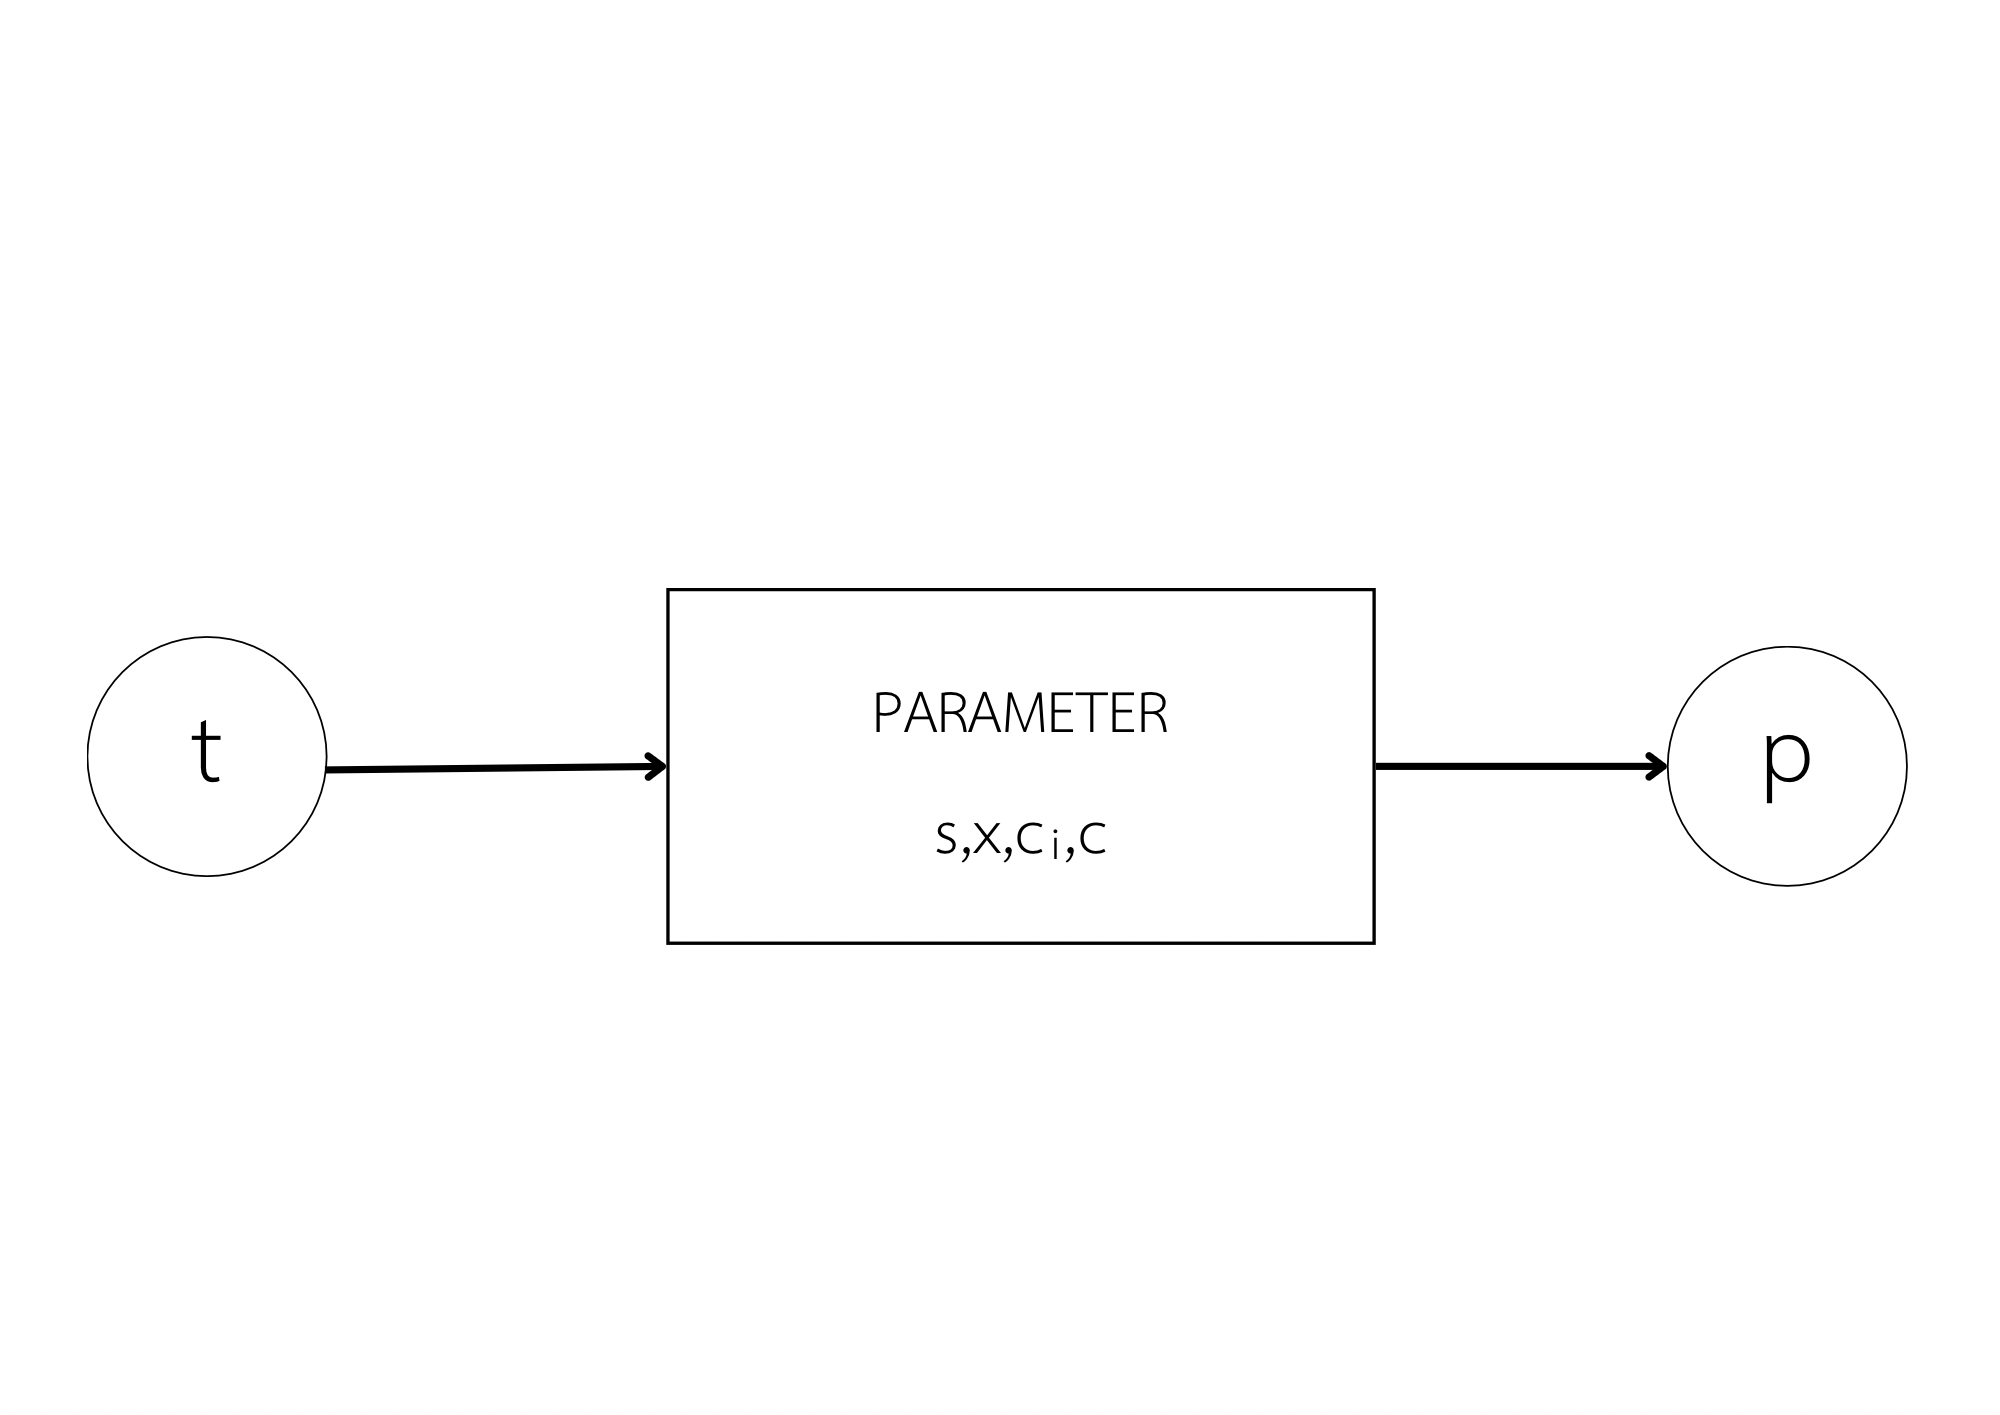
\includegraphics[scale=0.3]{KR.png}
	\caption{ภาพแสดงตัวแปรในโจทย์}
	\label{fig : graph2}
\end{figure}

\section{สมมติฐาน (Assumptions)} 
\begin{itemize}
	\item[-] แบบจําลองนี้สามารถให้คําตอบได้ว่าจะต้องขายกี่ชิ้นถึงจะได้กําไรและภายในระยะเวลากี่เดือน
	\item[-] ในการขายในแต่ละเดือนรายได้ต้องไม่ติดลบ
	\item[-] ต้องจำหน่ายออกให้ได้ทุกวัน
\end{itemize}

\section{ปัญหาในรูปคณิตศาสตร์ (Mathematical Problem)}\par
\hspace{0.5cm}\textbf{ทฤษฎีบท}
\begin{align*}
\text{ระยะเวลา} = \frac{\text{ต้นทุน}}{\text{ยอดขาย}}
\end{align*}
\begin{align*}
\text{กำไร} = \text{(ยอดขาย*ระยะเวลา)} - \text{ต้นทุน}
\end{align*}
\hspace{0.5cm}\underline{จากองค์ประกอบข้างต้น}
\begin{itemize}
	\item[-] ระยะเวลา $(t)$ เป็นตัวแปรนำเข้าที่บ่งบอกถึงระยะเวลาที่จะลงทุน เป็นเดือนหรือปี
	\item[-] ยอดขาย $(s)$ เป็นจำนวนเงินที่ขายได้ในแต่ละเดือน
	\item[-] ค่าต้นทุนต่อเดือน $(x)$ เป็นจำนวนเงินที่ใช้ในการผลิตสินค้าหรือบริการในแต่ละเดือน
	\item[-] ราคาขายครัวซองค์ $(c_i)$ เป็นราคาขายของสินค้าหรือบริการแต่ละชิ้นของครัวซองค์
	\item[-] จำนวนครัวซองค์ $(c)$ คือจำนวนของครัวซองค์ที่ขายได้ในแต่ละเดือน
	\item[-] ตัวแปรผลลัพธ์ $(p)$ คือกำไรที่ได้จากการดำเนินงานในแต่ละเดือน
\end{itemize}
\begin{itemize}
\item จากสมการ $p = (s)t - x$ บ่งบอกถึงวิธีการคำนวณกำไรโดยการลบค่าต้นทุนจากยอดขาย โดยกำหนดให้ $(t)$ เป็นระยะเวลาที่ลงทุน และ $(s)$ เป็นยอดขายในแต่ละเดือน และ $(x)$ เป็นค่าต้นทุนต่อเดือน จะได้ผลลัพธ์หรือกำไรที่ได้ในระยะเวลา t นั้น ๆ \par
\item จากสมการ $s = (c_i)\cdot (c)$ บ่งบอกถึงวิธีการคำนวณยอดขายโดยการคูณราคาขายต่อชิ้น $(c_i)$ กับจำนวนชิ้นที่ขายได้ $(c)$ ซึ่งนำไปคูณ 30 เพื่อที่จะได้จำนวนชิ้น/เดือน จะทำให้ได้ยอดขายทั้งหมด
\end{itemize}
ส่วน Solution 
การแก้สมการ $$(s)t - x > 0$$ เพื่อหาเงื่อนไขที่ต้องทำให้เป็นจริง:
\begin{align*}	
	(s)t - x &> 0
\end{align*}
เราจะนำ x มาบวกทั้งสองข้าง :
\begin{align*}	
	(s)t &> x
\end{align*}
และนำ 1/s มาคูณทั้งสองข้าง:
\begin{align*}	
	t &> \frac{x}{s}
\end{align*}
ซึ่งถ้าเราต้องการให้สมการนี้เป็นจริง เราจะต้องมี 
\begin{align*}	
	t &> \frac{x}{s}
\end{align*}
ดังนั้น เงื่อนไขที่ต้องทำให้สมการ $$(s)t - x > 0$$ เป็นจริงคือ 
\begin{align*}	
t จะต้อง >\frac{x}{s} นั่นคือ
\end{align*}
เราสามารถสรุปได้ว่า 
$$t จะต้อง> \frac{x}{s} $$
เพื่อให้สมการ $(s)t - x > 0$ เป็นจริง และจะได้ค่า $t$ คือเวลา

\subsection{แบบจำลองทางคณิตศาสตร์การลงทุนธุรกิจร้านครัวซองค์}
\begin{figure}[!h]
	\centering
	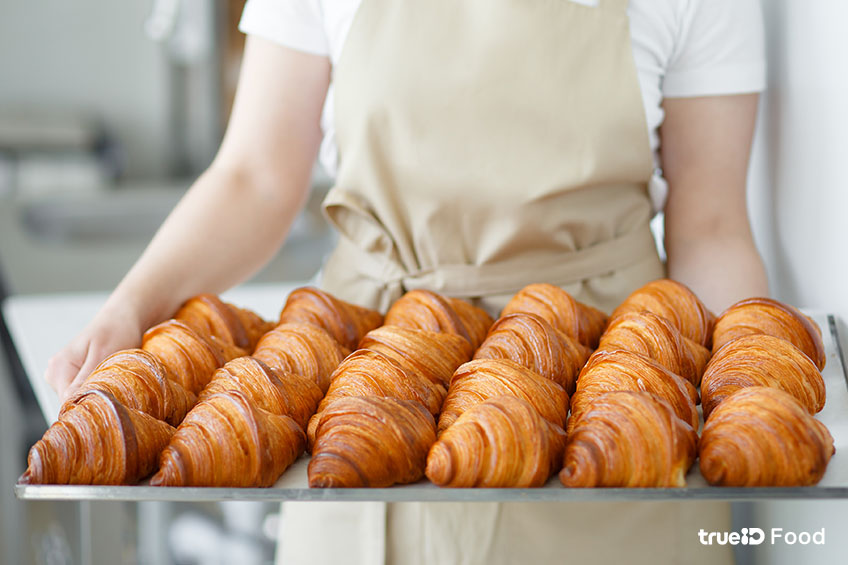
\includegraphics[scale=0.2]{DD.jpg}
	\caption{ภาพครัวซองค์ \cite{POPO}}
	\label{fig:graph3}
\end{figure}
จากปัญหาและสัญลักษณ์ข้างต้น สามารถเขียนปัญหาได้ในรูปแบบของคณิตศาสตร์ได้ดังนี้
กำหนดให้ ${c,c_i,s,x}\in\mathbb{R_{+}}$ และ ${p}\in\mathbb{R}$ จงหา 
${t}\in\mathbb{N}$ 
ที่ทำให้ $p>0$ เมื่อ
\begin{equation}
	p = (s)t - x 
\end{equation}
โดยที่ 
	$$s = (c_i)\cdot (c)$$
\textbf{Solution} เราจะได้กำไรเมื่อ
\begin{align}
(s)t - x &> 0 \\
(s)t &> x \\
t &>\frac{x}{s}
\end{align}


\chapter{ผลลัพธ์เชิงตัวเลข}
หลังจากการสืบค้นรวบรวมข้อมูลจริงแล้วนั้น สามารถคาดเดารายได้และต้นทุนได้ดังกรณี
ตัวอย่างดังต่อไปนี้
\section{การหาระยะเวลาการขายกี่เดือนถึงจะได้กำไร}
ราคาโดยเฉลี่ยต่อลูกค้า 1 คน $(c_i)$ 70 บาทต่อคน \\
จำนวนชิ้นที่ขาย $(c)$ โดยประมาณ 60ชิ้นต่อวัน หรือ 1,800 ชิ้นต่อเดือน \\
ค่าต้นทุนต่อเดือน $(x)$ 500,000 บาท \\
จากสมการที่ (3.1)\par 
\begin{equation} 
	p = (70)(1,800)t - 500,000 
\end{equation}
จากสมการที่ (3.4) จะได้ผลเฉลยคือ
\begin{align*}
t &> \frac{500,000}{(70)(1,800)} \\
t &> \frac{500,000}{126,000} \\
t &> 4 \\
\end{align*}
จะได้ว่าถ้าใน 1 วัน นางสาวเอขายได้วันละ $(c)$ 60 ชิ้น จะทำให้การลงทุนในการขายครัวซองค์นี้ใช้ระยะเวลาประมาณ 4 เดือน ถึงจะเริ่มได้กำไร
\section{โปรแกรมที่ใช้คำนวณ}
\begin{verbatim}
#หาระยะเวลา T
t = 4
# Input
c = 60 # จำนวนชิ้น

# Parameters
c_i = 70 # ราคาต่อชิ้น
x = 500000 # ค่าลงทุน

s = c_i * c  * 30  # ยอดขายรายเดือน
p = (s)*t - x  # กำไรต่อเดือน

# Output

# Report
print(f'ยอดขายรายเดือน: {s}')
print(f'กำไรต่อเดือน: {p}')

# ทดสอบเงื่อนไของผลเฉลย
T = x/s
print(f'Right Hand Side: {T}')
if  T < t :
    print('เงื่อนไขการได้กำไร : OK')
else:
    print('เงื่อนไขการได้กำไร : NOT OK T-T')
\end{verbatim}
\raggedright\begin{figure}[!ht]
    \centering
    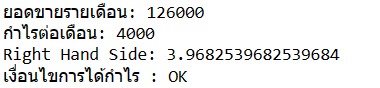
\includegraphics[scale=0.85]{A1.png}
    \caption{ผลลัพธ์จากโค้ดข้างต้น} 
\label{fig:mesh1}
\end{figure} 
*********************************************************************
\begin{verbatim}
import matplotlib.pyplot as plt

def cal_profit(t):
    # Parameters
    c_i = 70 # ราคาต่อชิ้น
    x = 500000 # ค่าลงทุน

    s = c_i * c  * 30  # ยอดขายรายเดือน


    # Output
    p = (s)* t - x  # กำไรต่อเดือน
    return p
\end{verbatim}
*********************************************************************
\begin{verbatim}
for t in range(0, 5):
    profit = cal_profit(t) 
    print(f'ต้องลงทุน {t} เดือน ถึงจะได้กำไร {profit}')
print('end')
\end{verbatim}
\begin{figure}[!ht]
    \centering
    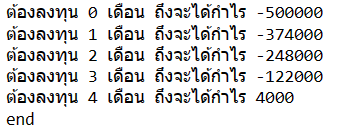
\includegraphics[scale=0.85]{A2.png}
    \caption{ผลลัพธ์จากโค้ดข้างต้น} 
\label{fig:mesh2}
\end{figure}
*********************************************************************
\begin{verbatim}
import numpy as np

def calculate_profit(s, t, x):
    return (s * t) - x

# สร้างข้อมูลจำลอง
np.random.seed(42)
num_samples = 1000
s_samples = np.random.uniform(10000, 50000, size=num_samples)  # สุ่มยอดขายรายเดือน (บาท/เดือน)
x_samples = np.random.uniform(5000, 20000, size=num_samples)   # สุ่มค่าต้นทุนต่อเดือน (บาท/เดือน)
t = 12  # ระยะเวลาลงทุน (เดือน)

# ประมวลผลข้อมูลแบบจำลอง
profits = calculate_profit(s_samples, t, x_samples)

# นับจำนวนที่กำไรเป็นบวก
positive_profits = sum(profits > 0)

# คำนวณสัดส่วนของกำไรเป็นบวก
positive_profit_percentage = (positive_profits / num_samples) * 100

print(f"จำนวนการทดลองที่ได้กำไร: {positive_profits}/{num_samples} ({positive_profit_percentage:.2f}%)")
\end{verbatim}
\begin{figure}[!ht]
    \centering
    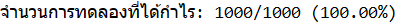
\includegraphics[scale=1.1]{A4.png}
    \caption{ผลลัพธ์จากโค้ดข้างต้น} 
\label{fig:mesh4}
\end{figure}
*********************************************************************
\begin{verbatim}
def main():
    # รับค่าพารามิเตอร์
    while True:
        try:
            ci = float(input("ราคาขายครัวซองค์ (บาท/ชิ้น): "))
            c = int(input("จำนวนครัวซองค์ที่ขาย (ชิ้น): "))
            t = int(input("ระยะเวลาลงทุน (เดือน): "))
            x = float(input("ค่าต้นทุนต่อเดือน (บาท/เดือน): "))
            break
        except ValueError:
            print("โปรดป้อนค่าที่เป็นจำนวนเต็มหรือจำนวนจริงเท่านั้น")

    #แสดงผลลัพธ์
    profit = calculate_profit(ci, c, t, x)
    print("กำไรต่อเดือน: {:.2f} บาท".format(profit))

if __name__ == "__main__":
    main()
\end{verbatim}
\begin{figure}[!ht]
    \centering
    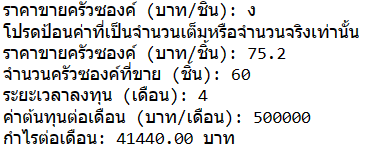
\includegraphics[scale=0.85]{A3.png}
    \caption{ผลลัพธ์จากโค้ดข้างต้น} 
\label{fig:mesh3}
\end{figure}
*********************************************************************
\begin{verbatim}
#พล็อตเทียบชิ้นว่าต้องใช้กี่ชิ้นถึงจะได้กำไร
#from ipywidgets import interact, interactive, fixed, interact_manual
import matplotlib.pyplot as plt
import math 
import ipywidgets as widgets
from IPython.display import display, clear_output
#ส่วนกำหนดเดือน
h = 60
#ส่วนป้อนข้อมูล
c = widgets.IntText(description='จำนวนชิ้น')
t = widgets.IntText(description='ระยะเวลาที่ลงทุน')
c_i = widgets.IntText(description='ราคาต่อชิ้น')
x = widgets.IntText(description='ค่าลงทุน')

def plotter(c,t,c_i,x):
    s = c_i * c  * 30  # ยอดขายรายเดือน
    
    list_p = []
    list_h = []
    
    for h1 in range(0,t+1):
        list_h.append(h1)

        p = (s)*h1 - x 
        list_p.append(p)
    plt.plot(list_h,list_p,label='M')
    plt.xlabel('Month') #ผลผลิต
    plt.ylabel('Profit')  #กำไร
    plt.grid()
    plt.legend()
    plt.show()
    
def calculate(r):
    with output:
        clear_output()
        display(plotter(c.value,t.value,c_i.value,x.value))

#ส่วนแสดงผล
ti = widgets.VBox([c,t,c_i,x])

calc_button = widgets.Button(description='Calculate')
calc_button.on_click(calculate)
output = widgets.Output()
outer = widgets.VBox([calc_button,output])
screen = widgets.HBox([ti,outer])
display(screen)
\end{verbatim}
\chapter{บทวิเคราะห์}
\textbf{ปัญหา:}นางสาวเอทำการลงทุนธุรกิจร้านขายครัวซองค์  ใช้ระยะเวลากี่เดือนถึงจะได้กำไร\\
	ในการลงทุนในธุรกิจร้านครัวซองค์นี้ ถ้ามีลูกค้าในแต่ละวัน 60 คน หรือต่อเดือน 1,800 คน จะทําให้การลงทุนในธุรกิจนี้ ใช้ระยะเวลาประมาณ 4 เดือน ถึงจะเริ่มได้กำไร \\
	(3.4) ในหน้าที่ 15

\begin{figure}[!ht]
    \centering
    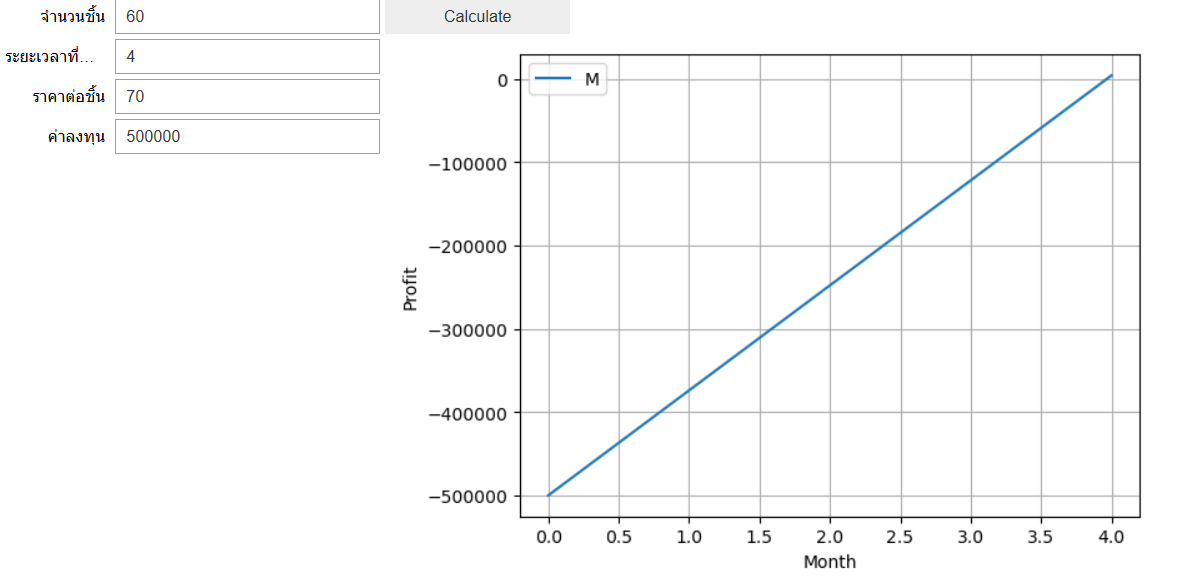
\includegraphics[scale=0.43]{B1.png}
    \caption{ปัญหาที่ 1} 
\label{fig:mesh1}
\end{figure}

\chapter{ผลสรุป}
จากการที่ได้ทำแบบจำลองทางคณิตศาสตร์ในการที่จะเริ่มลงทุนกับธุรกิจการขายครัวซองค์ เราจำเป็นต้องคำนึงถึงเงินลงทุนที่มีอยู่อย่างจำกัดเป็นหลักและต้องคำนึงถึงค่าสินค้าต่างๆ มีการสำรองค่าใช้จ่ายต่างๆเผื่อสำหรับกรณีฉุกเฉิน
ถ้าคุณมีเงินมากพอคุณก็สามารถเปิดร้านขายครัวซองค์ได้ และสามารถทำให้ได้กำไรโดยภายในปีนั้นได้
สิ่งที่ผู้จัดทำต้องการ คือการคำนวณผลกำไรในแต่ละเดือน และในแต่ละเดือนรายได้จะต้องไม่ติดลบ
สุดท้ายนี้ แบบจำลองทางคณิตศาสตร์ธุรกิจการขายครัวซองต์ ก็เป็นเพียงแบบจำลองตัวอย่างที่ใช้ประกอบการตัดสินใจในการลงทุนเท่านั้น ทั้งนี้อยู่ที่ความเห็นและความเหมาะสมของผู้ลงทุนแต่ละคนว่าจะลงทุนในธุรกิจนี้หรือไม่ เพราะการลงทุนมีความเสี่ยงควรศึกษาเพิ่มเติมให้มาก ก่อนจะดำเนินธุรกิจต่างๆไม่ว่าจะเป็นอะไรก็ตาม
 

 
\printbibliography
\end{document}